\subsection{Dead Reckoning}\label{subsec:Dead-Reckoning}
Dead Reckoning is simplest algorithm under test.
It implements only the prediction step of the Bayes filter shown in equation \ref{eq:bayes_prediction}.
A full diagram of the implemented dead reckoning algorithm is shown in Figure \ref{fig:dead_reckoning}.
The prediction step is implemented as a callback method when the Dead Reckoning node receives a \texttt{nav\_msgs/Odometry} message.

\begin{figure}[!htbp]
    \centering
    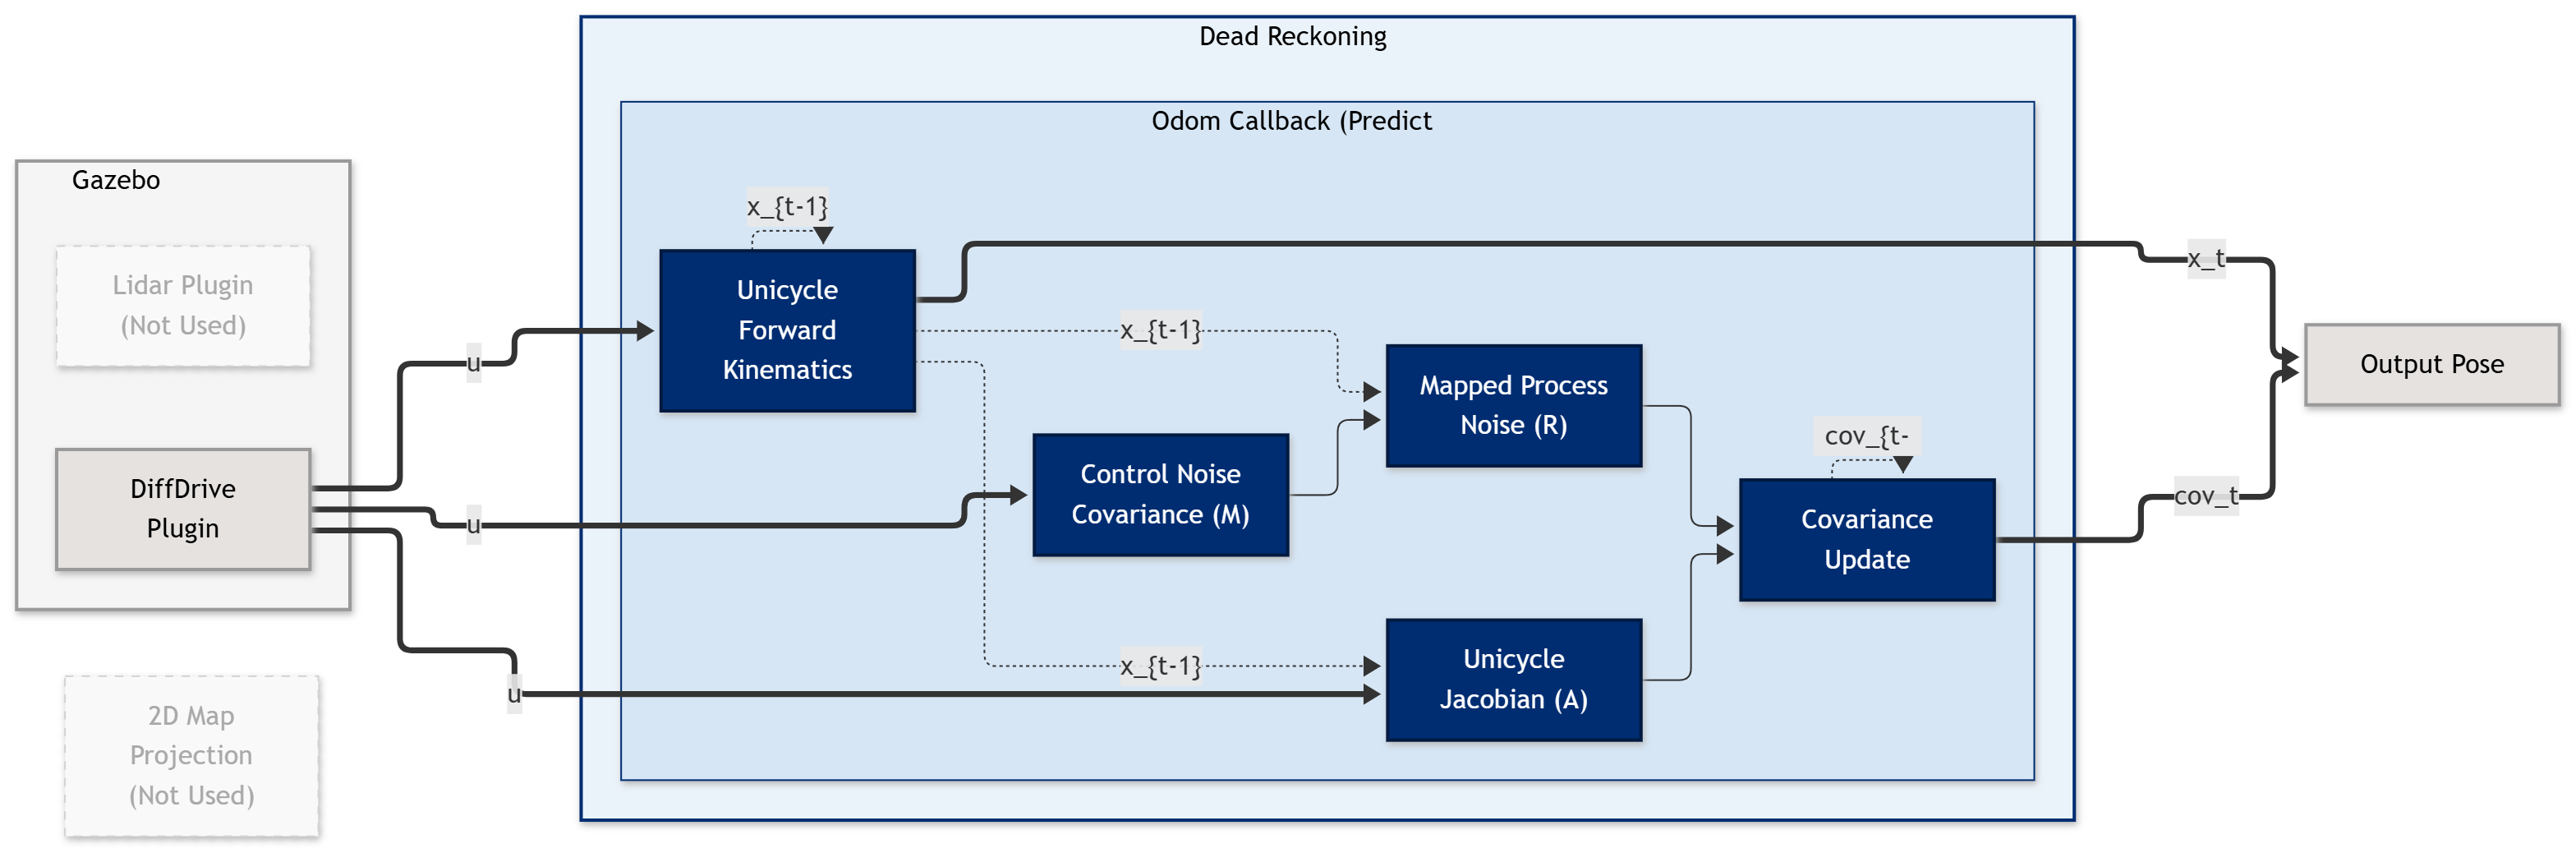
\includegraphics[width=\textwidth]{figures/dead_reckoning.png}
    \caption{Dead Reckoning Algorithm}
    \label{fig:dead_reckoning}
\end{figure}

\subsubsection{Prediction}\label{subsec:Dead-Reckoning:Prediction}
The algorithm begins by performing the forward kinematics described in Equation \ref{eq:discrete_unicycle_kinematics} to create a prediction of $\bar{\textbf{x}_t}$.
The previous state $\textbf{x}_{t-1}$ and raw Odometry message $\textbf{u}_{t}$ are used to calculate the state Jacobian $\textbf{A}_t$ shown in equation \ref{eq:state_jacobian_unicycle}.
The control noise covariance matrix $M_t$ can be calculated from the noises calculated in Equations \ref{eq:v-noise} and \ref{eq:omega-noise}:

\begin{equation} \label{eq:control_noise_covariance}
    M_t = \begin{bmatrix}
        \sigma_v^2 & 0 \\
        0 & \omega_v^2
    \end{bmatrix}
\end{equation}

The mapped process noise $R_t$ is then found using the control Jacobian as shown in Equation \ref{eq:mapped_process_noise}

\begin{equation} \label{eq:mapped_process_noise}
    R_t = G_t M_t G_t^T \Delta t
\end{equation}

Next, the covariance is updated as shown in Equation \ref{eq:dr_cov_update}.

\begin{equation} \label{eq:dr_cov_update}
    \bar{\Sigma}_t = A_t \Sigma_{t-1} A_t^T + R
\end{equation}

At the end of the predict step, the predicted values $\bar{\textbf{x}_t}$ and $\bar{\Sigma_t}$ are published as a \texttt{PoseWithCovarianceStamped} message.
The implementation of the Dead Reckoning node and algorithm can be found in Appendix \ref{subsec:DR implementation}.
